%!TEX root = ../../../thesis.tex
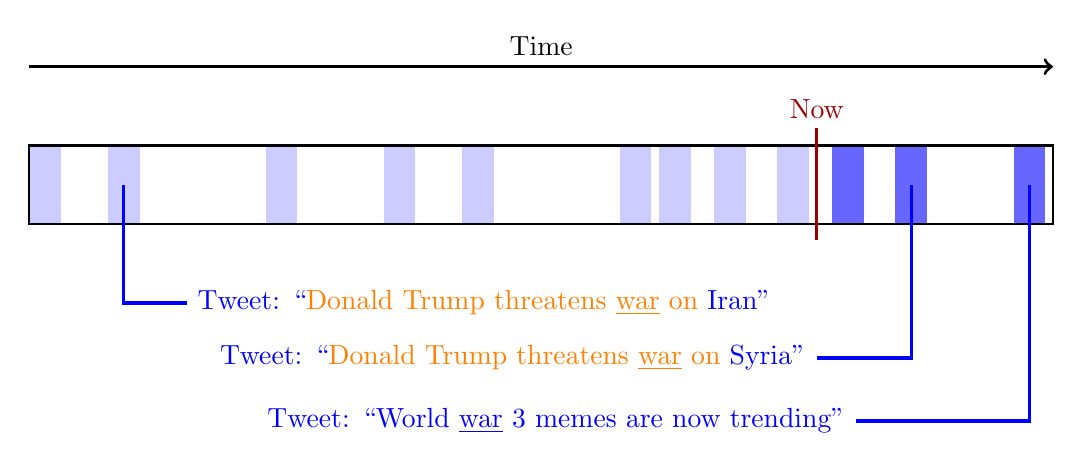
\begin{tikzpicture}

%% BLUE EVENTS
% Main
\draw [thick] (0,0) rectangle (13,1) ;

% Events
% Past Events
\foreach \x in {0, 1, 3, 4.5, 5.5, 7.5, 8, 8.7, 9.5}
{
	\fill[blue!20!white] (\x,0) rectangle ++(0.4,1);
}
% Future Events
\foreach \x in {10.2, 11, 12.5}
{
	\fill[blue!60!white] (\x,0) rectangle ++(0.4,1);
}

% Redraw Main Rectangle
\draw [thick] (0,0) rectangle (13,1) ;


% Time Arrow
\draw [very thick, ->] (0,2) -- (13,2) node[midway, above] {Time} ;



% Text
\draw[very thick,  blue] (1.2, 0.5 ) |- (2, -1) node [right] {Tweet: ``{\color{orange} Donald Trump threatens \underline{war} on} Iran''};
\draw[very thick,  blue] (11.2, 0.5 ) |- (10, -1.7) node [left] {Tweet: ``{\color{orange}Donald Trump threatens \underline{war} on} Syria''};
\draw[very thick,  blue] (12.7, 0.5 ) |- (10.5, -2.5) node [left] {Tweet: ``World \underline{war} 3 memes are now trending''};

% Now
\draw [red!60!black, very thick, shorten >= -0.6pt]        (10,-0.2 ) -- (10,1.2) node[above] {Now};

%		% Past brace
%	\usetikzlibrary{decorations.pathreplacing}
%	\draw [very thick, -, draw=black, decorate, decoration={brace,amplitude=10pt,mirror,raise=4pt} ] (9.8,1) -- (0.2,1)
%	node[midway, above, yshift = 14pt] {Past} ;
\end{tikzpicture}
